\section{Cluster Analysis}

\begin{figure}[!h]
    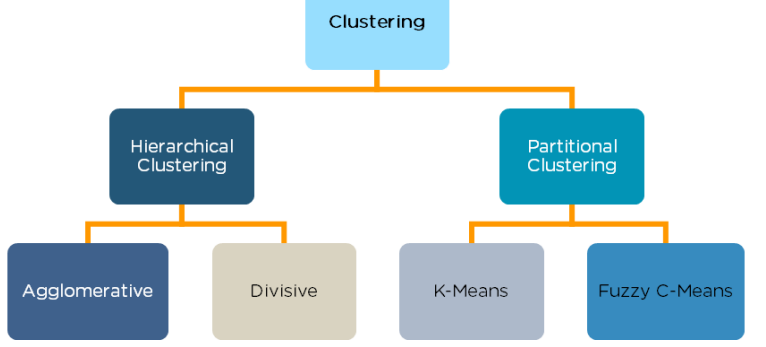
\includegraphics[width = \columnwidth]{figures/11/ClusteringOverview.png}   
\end{figure}
Clustering = Finding groups in data

Problem: given \(n\) data points, separate them into \(K\) clusters.
\begin{table}[!h]
    \begin{tabular}{ll}
    \(n\) &  number of data points\\
    \(K\) &  number of clusters \((K << n)\)\\
    \(\Delta\) &  a partition, \(\Delta = \{C_1,C_2,\dots,C_K\}\)\\
    \(\mathcal{L}(\Delta)\) & loss of \(\Delta\) to be minimized
    \end{tabular}
\end{table}

\subsection{Taxonomy of Clustering}
Hard clustering: Each data point is assigned a unique cluster:\(\Delta\)

Soft clustering: Each data point \(i\) is assigned a probability that it is in cluster \(k\):

Parametric clustering: \(k\) known

Non-parametric: \(k\) determined by algorithm
\subsection{Hierarchical Clustering}
Hierarchical Clustering (HCA) seeks to build a hierarchy of clusters.
Strategies for hierarchical clustering generally fall into two types:
\begin{itemize}
    \item Agglomerative: This is a bottom-up approach: each observation starts in its own cluster, and pairs of clusters are merged as one moves up their hierarchy.
    \item Divisive: This is a top-down approach: all observations start in one cluster, and splits are performed recursively as one moves down the hierarchy.
\end{itemize}
We start with \(N\) datapoints that initially form \(N\) clusters.
The two clusters with the smallest linkage are fused togther to form \(N - 1\) clusters.
This is repeated until there is only one single cluster.
\[
(i,j)_{fused} = \arg\min_{i \neq j}\{D_{link}(C_i,C_j)\}
\]
\subsubsection{Linkage criteria}
The linkage citerion determines together with a metric \(d(x,y)\) when two clusters \(A\) and \(B\) should be merged together in hierarchical clustering (fusion criterium)
\begin{table}[]
    \begin{tabular}{ll}
    Maximum(complete) &  \(\max\{d(a,b): a\in A,b\in B\}\)\\
    Minimum(single) &  \(\min\{d(a,b):a\in A,b\in B\}\)\\
    Mean(average) &  \(\frac{1}{|A|\cdot|B|}\sum_{a\in A}\sum_{b\in B}d(a,b)\)\\
    Centroid & \(||c_s-c_t||\)
    \end{tabular}
\end{table}

where \(c_s\) and \(c_t\) are the centroids of clusters \(s\) and \(t\), respectively.
\begin{figure}[!h]
    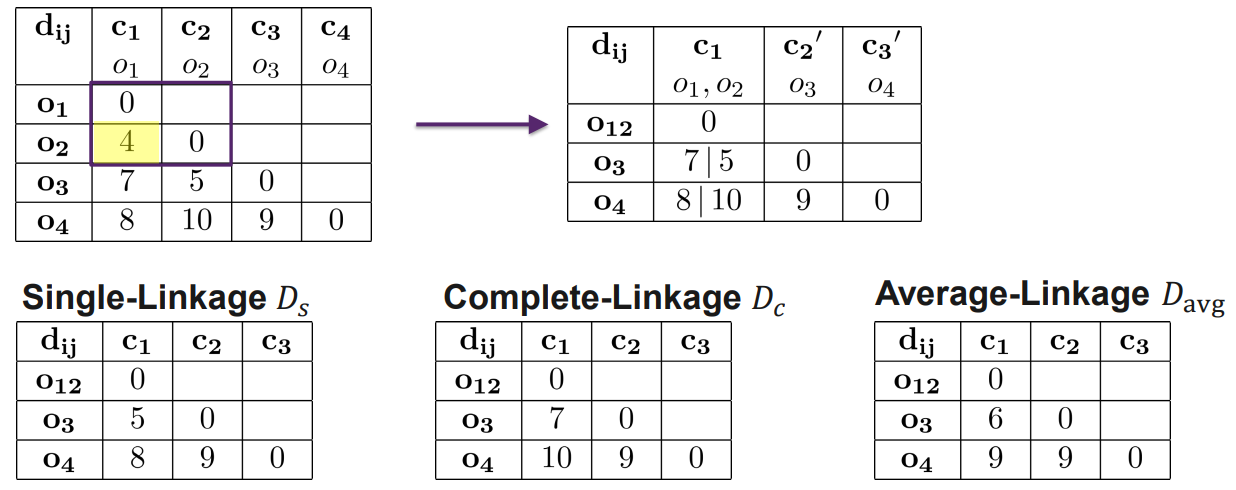
\includegraphics[width = \columnwidth]{figures/11/ExampleHCA.png}    
\end{figure}

\subsubsection{Basic Algorithm}
Input:
\begin{itemize}
    \item Distance matrix \(D\) data points (size \(n\times n\))
    \item fucntion \(d(a,b)\) to compute a distance between clusters (usually takes \(D\) as input)
\end{itemize}
Initialization: Clustering \(\mathcal{C}^{(0)} = \{C_1^{(0)},C_2^{(0)},\dots,C_n^{(0)}\} = \{i\}\)

While the current number of clusters is \(>1\):
\begin{itemize}
    \item find the two clusters which have the smallest linkage to each other
    \item merge them to one cluster
\end{itemize}
Ouput: Resulting Dendrogram: The Dendrogram is a tree that represent the hierarchical division of the data set \(O\) into ever smaller subsets.


Dendrograms cannot tell you how many clusters you should have: Interpretation of this kind is justified only when the ultrametric tree inequality holds, which is very rare.
\begin{figure}[!h]
    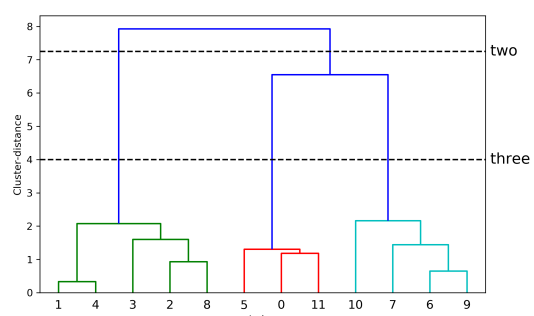
\includegraphics[width = \columnwidth]{figures/11/Dendrogram.png}
\end{figure}


\subsection{K-means}
\begin{figure}[!h]
    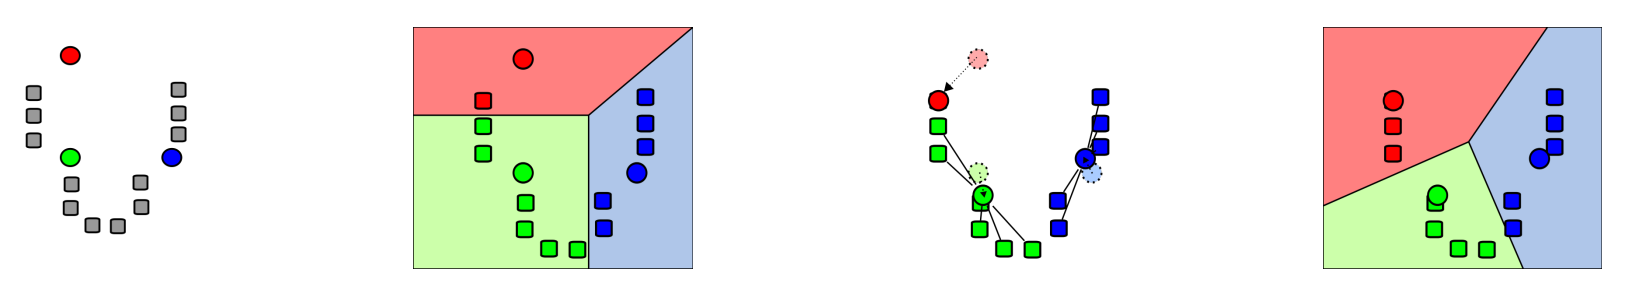
\includegraphics[width = \columnwidth]{figures/11/KMeansExample.png}
\end{figure}
The standard algorithem is non-probabilistic EM.
The problem is that k-means is very sensitive to the choice of \(k\), even with correct \(k\) it may converge to wrong local Minimum.
\subsubsection{K-means algorithm}
Input: Data \(\mathcal{D} = \{x_i\}_{i = 1:N}\), number of clusters \(K\)

Initialize: centers \(\mu_1,\mu_2,\dots,\mu_k \in \mathbb{R}^d\) at random

Iterate until convergence:
\begin{enumerate}
    \item for \(i = 1:n\): \(k(i) = \arg\min_k||x_i-\mu_i||\)(assign points to cluster \(\rightarrow\) new clustering)
    
    \item for \(k = 1:K\): \(\mu_k = \frac{1}{|C_k|}\sum_{i \in C_k}x_i\) (recalcuate centers)
\end{enumerate}
Convergence: if \(\Delta\) does not change after iteration \(m\), it will never change after that.

How to pick starting points?:
\begin{itemize}
    \item Random initialization: Randomly choose some data points as starting centers.
    \item Forgy method: Chooses \(k\) observations from the dataset and uses these as the initial means.
    \item Random Partition: Randomly assignes a cluster to each observation an then proceeds to the update step, thus computing the initial mean to be the centroid of the clusters randomly assigned points.
    \item K-means++: The algorithm is guaranteed to find a solution that is \(O(\log k)\) competitive to the optimal k-means solution.
\end{itemize}
\subsubsection{K-means cost function}
The distortion(least-squares) can also be expressed as sum of (squared) intracluster distances:
\[
\mathcal{L}(\Delta) = \frac{1}{2}\sum_{k = 1}^K\sum_{i\in C_k}||x_i - x_j||^2 + \text{const}
\]
\subsubsection{Limitations of K-means: Non-globular shapes}
\begin{enumerate}
    \item Inertia W makes the assumption that clusters are convex and isotropic.
    \item Inertia W is not a normalized metric.
\end{enumerate}
\subsubsection{More variants of K-means}
\begin{itemize}
    \item K-medians
    \item weighted K-means: weighted data points
    \item kernel-k-means
    \item soft K-means: soft assignments (in form of probability)
\end{itemize}

\subsubsection{How shall we choose \(k\)}
\begin{itemize}
    \item Basic Elbow method
    \item Try a range of \(K\) values and plot average distance to centers
    \item Silhoutte
    \item Cross-Validation
    \item Information theoretic perspective: NMI,BIC and AIC
\end{itemize}

\subsubsection*{Silhoutte Score}
A graphical method to select \(k\).
Given K and K clusters, given any data point \(i\), let \(a_i\) be the average distance or dissimilarity of \(i\) with all other points in the same cluster.
\(a_i\) measures how well \(i\) fits into its own cluster.
\(b_i\) is the smallest average distance(Euclidean distance) of \(i\) to other clusters.

Silhouette score \(s_i \in \left[-1,1\right]\):
\[
s_i = \frac{b_i - a_i}{\max(b_i,a_i)}
\]
\(s_i\approx 1\): point \(i\) is in a tight cluster and far away from other clusters

\(s_i\approx -1\): point \(i\) is in a loose cluster and close to other clusters

Maximize \(\frac{1}{n}\sum_{i = 1}^n s_i\) over \(k\).


